% Artigo final (Entrega parte 2) - Disciplina de Dados Categóricos
% Autora da disciplina: Profa. Ana Julia Alves Câmara (UFES)

\documentclass[12pt]{article}

% Pacotes básicos
\usepackage[utf8]{inputenc}
\usepackage[T1]{fontenc}
\usepackage[brazilian]{babel}
\usepackage{amsmath, amssymb}
\usepackage{graphicx}
\usepackage{booktabs}
\usepackage{setspace}
\usepackage{geometry}
\usepackage{hyperref}
\usepackage{xurl} % quebra URLs longas na bibliografia em qualquer ponto

\usepackage{biblatex} %Imports biblatex package
\addbibresource{ref.bib} %Import the bibliography file

\usepackage{tabularx}
\usepackage{makecell}

\geometry{margin=2.5cm}
\onehalfspacing
\setlength{\emergencystretch}{3em} % evita overfull em títulos/URLs longos da bibliografia

% Informações do artigo
\title{Distinção entre as áreas dos cursos de graduação ofertados pelas redes pública e privada no Brasil}
\author{Nathália Nunes \and João Gabriel \and Rafael Jordane}
\date{Disciplina: Dados Categóricos \\
Departamento de Estatística -- UFES \\
\today}

\begin{document}

\maketitle

% ---------------------------------------------------------------------------
% RESUMO (Etapa 6 do plano de escrita)
% ---------------------------------------------------------------------------

\begin{abstract}
\noindent Este trabalho investiga se há distinção clara entre os cursos de graduação ofertados pela rede pública e pela rede privada no Brasil. Usamos a base do Censo da Educação Superior 2024 (INEP), com 720.349 cursos, dos quais 97,2\% são da rede privada e 2,8\% da pública. Aplicamos três métodos: teste qui-quadrado com V de Cramér, regressão logística e modelo log-linear. A distinção existe, e o eixo mais forte não é a área do curso, é a modalidade de ensino: a associação entre rede e modalidade tem V de Cramér de 0,395, contra 0,128 para a área, e a EAD é o fator que mais associa um curso à rede privada (razão de chances de 0,033). O modelo log-linear mostra que esse contraste depende do grau acadêmico, sendo mais extremo no Tecnológico. A distinção é de estratégia de oferta, e não de conteúdo do curso.

\vspace{1em}
\noindent\textbf{Palavras-chave:} educação superior; rede pública e privada; dados categóricos; qui-quadrado; regressão logística; modelos log-lineares.
\end{abstract}

% ---------------------------------------------------------------------------
% INTRODUÇÃO E DADOS (Etapa 4: revisão do texto da entrega 1)
% ---------------------------------------------------------------------------

\section{Introdução}

A educação superior no Brasil cresce a cada ano. Segundo dados do Censo da Educação Superior (2024), entre 2014 e 2024 a matrícula na educação superior aumentou 30,5\%, sendo de 2,7\% o crescimento de 2023 para 2024. Se até a metade do Século XIX a formação superior se concentrava em áreas como medicina, engenharia civil e direito, com cerca de 5 cursos em todo o território brasileiro \parencite{cunhaUniversidadeTemporaEnsino2007}, em 2024 o número de cursos de graduação ofertados por instituições públicas e privadas no Brasil chega a 45.776, das mais diversas áreas (INEP, 2025). O Censo da Educação Superior cumpre um papel importante de documentação desse crescimento, registrando com detalhes o perfil da educação brasileira a cada ano e permitindo que esses dados sirvam de base para estudos sobre o tema.

Embora alguns autores como \textcite{motaEDUCACAOSUPERIOREM2012} tenham direcionado pesquisas para a projeção da oferta de vagas em áreas específicas como o Turismo, o campo social traz contribuições ainda mais abrangentes quando a disparidade entre a educação superior pública e privada é posta sob análise. Um exemplo é o tema da mercantilização da educação, tratado por \textcite{carvalhoMercantilizacaoEducacaoSuperior2013}, que ainda na década passada discutia o impacto do mercado financeiro e das grandes empresas na educação brasileira, apontando um contraponto entre o ensino público e o privado.

Compreendendo a complexidade da educação superior como uma instituição social indissociável das demais questões que cercam a sociedade brasileira, o presente estudo busca investigar se é possível identificar uma distinção clara entre os cursos de graduação ofertados pelas instituições públicas e privadas no Brasil. A distinção pode se dar em mais de um eixo, então além da área do curso examinamos também o grau acadêmico e a modalidade de ensino. O objetivo é que os resultados sirvam de apoio a pesquisas que busquem identificar mais a fundo os fatores que afetam a oferta de cursos no país.

\section{Base de Dados}

Para responder à pergunta proposta, utilizou-se a base do Censo da Educação Superior de 2024, pesquisa estatística anual coordenada pelo Instituto Nacional de Estudos e Pesquisas Educacionais Anísio Teixeira (INEP) em articulação com as Instituições de Educação Superior (IES) brasileiras. Os microdados foram coletados a partir do cadastro do Sistema e-MEC, abrangendo informações sobre instituições, cursos, infraestrutura, vagas, matrículas, ingressantes, concluintes e docentes, e são amplamente reconhecidos como o instrumento mais completo de caracterização do sistema de educação superior no país.

Para este estudo, foram selecionados os microdados do Cadastro de Cursos disponibilizados publicamente pelo INEP. O arquivo original contém 720.349 observações (registros de cursos), descritas por um conjunto de 223 variáveis. A população alvo da pesquisa foram todos os cursos de graduação registrados no Brasil que declararam informações ao censo no ano de referência. Os resultados das análises refletem a base após a aplicação dos filtros de seleção descritos a seguir.

\subsection{Critérios de Seleção e Variáveis Analisadas}

O processo de delimitação da base foi conduzido em duas etapas principais:

\begin{enumerate}
    \item Filtro por nível acadêmico: foram retidos exclusivamente os registros de cursos de graduação (bacharelado, licenciatura e tecnólogos), excluindo-se todos os cursos de pós-graduação (lato e stricto sensu). Este procedimento reduziu o escopo da análise ao objeto central da pesquisa.
    \item Seleção de variáveis: das 223 variáveis disponíveis, optou-se por um conjunto reduzido e focado nas dimensões de interesse. As variáveis selecionadas, com suas respectivas definições operacionais, são apresentadas na Tabela~\ref{tab:variaveis}.
\end{enumerate}

\begin{table}[h]
\centering
\begin{tabularx}{\linewidth}{ X  X }
  \hline
  \thead{Variável} & \thead{Descrição / Categoria analisada} \\
  \hline
Rede de Ensino & Classificação binária da IES como pública ou privada. \\
  \hline
Categoria Administrativa & Subdivisão detalhada da rede (ex.: Federal, Estadual, Municipal, Privada com fins lucrativos, Privada sem fins lucrativos). \\
  \hline
Área Geral & Nome da área geral do curso, conforme adaptação brasileira da Classificação Internacional Normalizada da Educação (ISCED-F) da UNESCO. \\
  \hline
Área Específica & Nome da área específica do curso (segundo nível hierárquico da classificação CINE). \\
  \hline
Área Detalhada & Nome da área detalhada do curso (terceiro nível hierárquico da classificação CINE). \\
  \hline
Nível Acadêmico & Tipo de curso (utilizado apenas para filtrar cursos de graduação). \\
  \hline
Código do Curso & Código único de identificação do curso no Cadastro Nacional de Cursos e Instituições da Educação Superior (Cadastro e-MEC). \\
  \hline
Nome do Curso & Denominação oficial do curso. \\
  \hline
\end{tabularx}
\caption{Variáveis selecionadas e suas definições operacionais. Fonte: elaboração própria com base na documentação do Censo da Educação Superior 2024 (INEP, 2025).}
\label{tab:variaveis}
\end{table}

\section{Análise exploratória}

A base tem 720.349 observações. Dentre as ofertas de cursos registradas, 700.198 (97,20\%) pertencem à rede privada e 20.151 (2,80\%) à rede pública.

\subsection{Distribuição das áreas gerais por rede}

A Tabela~\ref{tab:area-rede} apresenta a distribuição das áreas gerais CINE dentro de cada rede, ordenada pela diferença em pontos percentuais (p.p.) entre pública e privada.

\begin{table}[h]
\centering
\small
\begin{tabular}{lrrr}
\toprule
Área Geral & Privada (\%) & Pública (\%) & Dif. (Pub $-$ Priv) \\
\midrule
Educação & 19,63 & 43,65 & $+$24,02 \\
Engenharia, produção e construção & 8,94 & 12,83 & $+$3,89 \\
Agricultura, silvicultura, pesca e vet. & 1,09 & 3,46 & $+$2,37 \\
Ciências naturais, matemática e estat. & 1,33 & 3,37 & $+$2,04 \\
Programas básicos & 0,25 & 1,32 & $+$1,07 \\
Ciências sociais, comunicação e inf. & 4,46 & 3,28 & $-$1,18 \\
Computação e TIC & 10,21 & 8,20 & $-$2,01 \\
Artes e humanidades & 5,90 & 3,21 & $-$2,69 \\
Serviços & 7,01 & 1,29 & $-$5,72 \\
Saúde e bem-estar & 11,56 & 4,78 & $-$6,78 \\
Negócios, administração e direito & 29,62 & 14,61 & $-$15,01 \\
\bottomrule
\end{tabular}
\caption{Distribuição percentual das áreas gerais dentro de cada rede de ensino. Diferenças positivas indicam áreas proporcionalmente mais presentes na rede pública; negativas, na privada.}
\label{tab:area-rede}
\end{table}

O curso típico da rede privada está em \textit{Negócios, administração e direito} (29,6\%), enquanto o da rede pública está em \textit{Educação} (43,6\%). A rede pública é, no conjunto, mais concentrada (Educação responde por quase metade do total), enquanto a privada se distribui entre Negócios, Educação, Saúde, TIC e Serviços.

Em termos de perfil:
\begin{itemize}
    \item \textbf{Áreas com maior peso na rede pública:} Educação ($+$24,0~p.p.), Engenharias ($+$3,9), Agricultura/Veterinária ($+$2,4), Ciências naturais e matemática ($+$2,0), Programas básicos ($+$1,1). Configura-se um perfil voltado à formação de professores, ciências básicas e áreas tradicionalmente vinculadas à pesquisa.
    \item \textbf{Áreas com maior peso na rede privada:} Negócios/Direito ($-$15,0~p.p.), Saúde ($-$6,8), Serviços ($-$5,7), Artes/Humanidades ($-$2,7), Computação/TIC ($-$2,0). Perfil compatível com graduações de forte demanda no mercado de trabalho.
\end{itemize}

\subsection{Variáveis complementares}

A análise das áreas não pode ser dissociada de outras dimensões em que as redes diferem fortemente.

\paragraph{Grau acadêmico.} A rede privada é majoritariamente composta por tecnólogos (48,0\%), enquanto a pública se divide quase igualmente entre bacharelado (42,8\%) e licenciatura (43,6\%). Como a licenciatura se concentra em \textit{Educação} e os cursos tecnólogos em \textit{Negócios} e \textit{TIC}, parte relevante da diferença observada em áreas pode ser absorvida pelo grau. A Figura~\ref{fig:grau-bi} ilustra essa assimetria.

\begin{figure}[h]
\centering
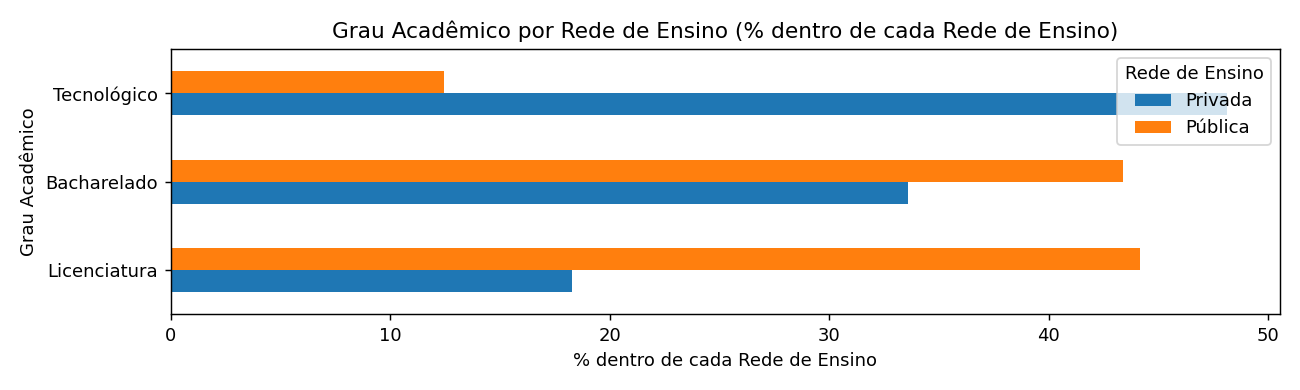
\includegraphics[width=0.8\textwidth]{descritiva_plots/bi_TP_GRAU_ACADEMICO_por_rede.png}
\caption{Distribuição do grau acadêmico (Bacharelado, Licenciatura, Tecnológico) dentro de cada rede de ensino.}
\label{fig:grau-bi}
\end{figure}

\paragraph{Modalidade de ensino.} A discrepância é acentuada: 96,6\% da oferta privada está em EAD, contra 45,2\% na pública (Figura~\ref{fig:modalidade-bi}). Como a EAD se concentra em certas áreas (TIC, Negócios, Educação a distância), a modalidade é um segundo eixo a ser controlado.

\begin{figure}[h]
\centering
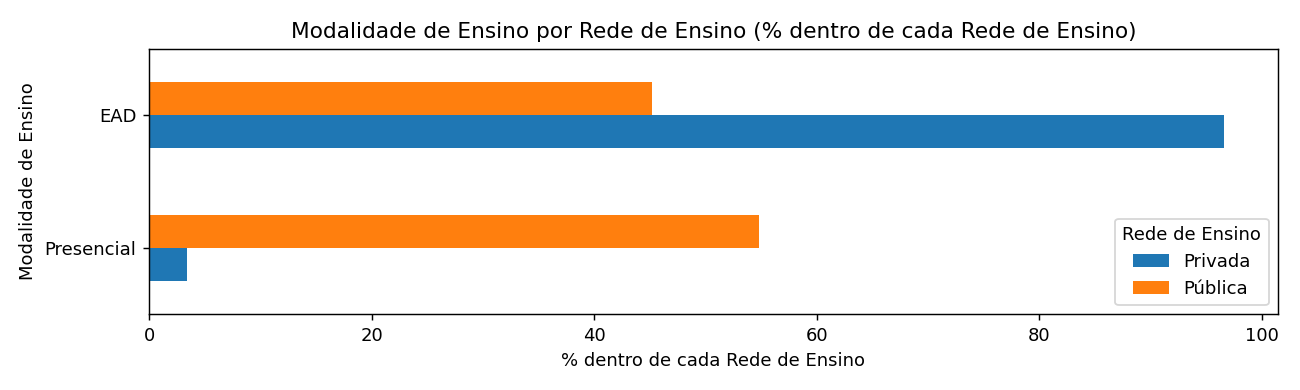
\includegraphics[width=0.6\textwidth]{descritiva_plots/bi_TP_MODALIDADE_ENSINO_por_rede.png}
\caption{Distribuição da modalidade de ensino (Presencial vs.\ EAD) dentro de cada rede.}
\label{fig:modalidade-bi}
\end{figure}

\subsection{Geografia}

A distribuição regional (Figura~\ref{fig:regiao-bi}) mostra que o Sudeste é o eixo principal em ambas as redes (cerca de 40\% das ofertas). As diferenças regionais mais marcantes são o \textit{Sul mais privado} (22,1\% vs.\ 13,7\%) e o \textit{Nordeste mais público} (25,6\% vs.\ 19,6\%).

\begin{figure}[h]
\centering
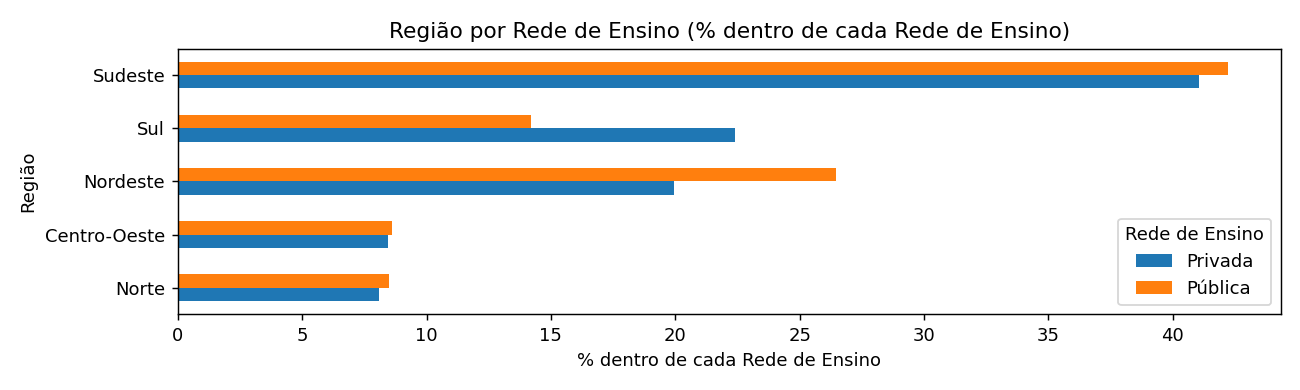
\includegraphics[width=0.7\textwidth]{descritiva_plots/bi_NO_REGIAO_por_rede.png}
\caption{Distribuição regional da oferta de cursos dentro de cada rede de ensino.}
\label{fig:regiao-bi}
\end{figure}

% ---------------------------------------------------------------------------
% METODOLOGIA (Etapa 1 do plano de escrita)
% ---------------------------------------------------------------------------

\section{Metodologia}

A pergunta do trabalho é se a rede de ensino (pública ou privada) está associada ao perfil dos cursos de graduação que cada rede oferece, e, se estiver, em qual característica essa distinção se concentra. As características examinadas são categóricas: a área geral do curso na classificação CINE (11 categorias), o grau acadêmico (Bacharelado, Licenciatura, Tecnológico) e a modalidade de ensino (Presencial ou EAD). Para responder a essa pergunta usamos três técnicas, aplicadas na ordem em que a análise foi ficando mais exigente. Primeiro o teste qui-quadrado, que mede a associação entre a rede e uma característica de cada vez. Depois a regressão logística, que estima o efeito de cada característica sobre a chance de um curso ser público controlando as demais ao mesmo tempo. Por último o modelo log-linear, que trata rede, grau e modalidade sem eleger nenhuma delas como resposta. Todas as análises foram feitas em R sobre a base do Censo da Educação Superior 2024 (INEP).

\subsection{Teste qui-quadrado, V de Cramér e resíduos padronizados}

O teste qui-quadrado de Pearson responde à primeira parte da pergunta: a rede e cada característica são independentes, ou há associação entre elas? Para cada característica montamos uma tabela de contingência cruzando a rede (2 linhas) com as categorias da característica ($R$ colunas) e comparamos a frequência observada em cada célula, $n_{ij}$, com a frequência que seria esperada se as duas variáveis fossem independentes,

\begin{equation}
e_{ij} = \frac{n_{i+}\,n_{+j}}{n}.
\end{equation}

A estatística soma essa discrepância sobre todas as células e segue uma distribuição $\chi^2$ com $(I-1)(R-1)$ graus de liberdade sob a hipótese de independência:

\begin{equation}
\chi^2 = \sum_{i=1}^{I}\sum_{j=1}^{R} \frac{(n_{ij}-e_{ij})^2}{e_{ij}}.
\end{equation}

A base tem cerca de 706 mil cursos, então todas as frequências esperadas ficam muito acima do mínimo de $e_{ij} \geq 5$ que a aproximação exige, e não foi preciso recorrer à correção de Yates nem ao teste exato de Fisher, que existem para tabelas com contagens baixas. O mesmo tamanho de amostra traz um problema conhecido: com $n$ tão grande, o $\chi^2$ fica inflado e o p-valor tende a zero mesmo quando a associação é fraca, de forma que a significância sozinha não informa a força da relação. Por isso reportamos, junto do teste, o V de Cramér, que normaliza o $\chi^2$ pelo tamanho da amostra e pela dimensão da tabela e varia de 0 (nenhuma associação) a 1 (associação perfeita):

\begin{equation}
V = \sqrt{\frac{\chi^2}{n\,\bigl(\min(I,R)-1\bigr)}}.
\end{equation}

O V de Cramér diz o quanto rede e característica estão associadas, mas não onde essa associação se concentra. Para localizar as células responsáveis pelo desvio de independência usamos o resíduo padronizado de Pearson,

\begin{equation}
r_{ij} = \frac{n_{ij}-e_{ij}}{\sqrt{e_{ij}}},
\end{equation}

e tratamos como relevante toda célula com $|r_{ij}| > 2$. Resíduo positivo indica mais cursos naquela combinação de rede e categoria do que a independência preveria; resíduo negativo indica menos. Os três testes, as três medidas de V de Cramér e os resíduos estão em \texttt{metodo1\_qui\_quadrado.R}.

\subsection{Regressão logística binária}

O teste qui-quadrado trata uma característica por vez e não separa efeitos que andam juntos. Grau, modalidade e área estão entrelaçados nesta base (a licenciatura concentra-se em Educação, a EAD concentra-se em certas áreas), então uma associação entre rede e área pode ser, em parte, reflexo da modalidade. A regressão logística responde a uma pergunta mais fina: controlando área, grau, modalidade e região ao mesmo tempo, qual característica mais distingue a rede pública da privada? Definimos a resposta binária $Y=1$ para curso da rede pública e modelamos o logaritmo da chance (logito) como função linear dos preditores:

\begin{equation}
\log\!\left(\frac{\pi(x)}{1-\pi(x)}\right) = \beta_0 + \beta_1 x_1 + \dots + \beta_p x_p,
\qquad
\pi(x) = \frac{e^{\,\beta_0 + \beta_1 x_1 + \dots + \beta_p x_p}}{1 + e^{\,\beta_0 + \beta_1 x_1 + \dots + \beta_p x_p}}.
\end{equation}

O logito garante que a probabilidade estimada fique entre 0 e 1, e os parâmetros são estimados por máxima verossimilhança. Cada coeficiente, exponenciado, é uma razão de chances (odds ratio), $\text{OR}_j = e^{\beta_j}$, que compara a chance de um curso ser público em uma categoria contra a chance na categoria de referência: $\text{OR}=1$ indica ausência de associação, valores acima de 1 associam a categoria à rede pública e abaixo de 1 à privada. O modelo ajustado foi

{\small
\begin{verbatim}
glm(rede_bin ~ area_geral + grau * modalidade + regiao,
    family = binomial)
\end{verbatim}
}

com Negócios/administração/direito, Bacharelado, Presencial e Sudeste como categorias de referência. O termo \texttt{grau * modalidade} entra porque suspeitamos que o efeito da modalidade sobre a chance de ser público não é o mesmo em todos os graus (o peso da EAD na rede privada varia entre bacharelado, licenciatura e tecnólogo), e um modelo só com efeitos principais não conseguiria representar isso. Ajustamos o modelo sobre os casos completos e os intervalos de confiança de 95\% das razões de chance são de Wald, escolha justificada pelo custo de calcular o intervalo por perfil de verossimilhança em uma base desse tamanho, onde a aproximação de Wald é boa. O código está em \texttt{metodo2\_regressao\_logistica.R}.

\subsection{Modelo log-linear}

A regressão logística obriga a eleger uma variável como resposta e a tratar as outras como preditoras. Isso cria uma dificuldade quando dois preditores quase coincidem, como grau Licenciatura e área Educação nesta base, porque o modelo não consegue separar os efeitos e o coeficiente correspondente sai com erro padrão inflado. O modelo log-linear contorna esse problema tratando as variáveis de forma simétrica: nenhuma é resposta, e o que se modela é o logaritmo da contagem esperada de cada célula. Montamos a tabela de três vias Rede $\times$ Grau $\times$ Modalidade (dimensão $2 \times 3 \times 2$) e ajustamos o modelo saturado, que inclui os três efeitos principais, as três interações de segunda ordem e a interação tripla:

\begin{equation}
\log(\mu_{ijk}) = \lambda + \lambda_i^{R} + \lambda_j^{G} + \lambda_k^{M} + \lambda_{ij}^{RG} + \lambda_{ik}^{RM} + \lambda_{jk}^{GM} + \lambda_{ijk}^{RGM}.
\end{equation}

É um GLM da família Poisson com função de ligação logarítmica, ajustado por

{\small
\begin{verbatim}
glm(Freq ~ rede * grau * modalidade, family = poisson)
\end{verbatim}
}

\noindent A pergunta aqui é se a interação tripla $\lambda_{ijk}^{RGM}$ pode ser removida sem prejudicar o ajuste, ou seja, se a associação entre rede e modalidade é a mesma nos três graus. Comparamos o modelo saturado com o modelo reduzido sem esse termo pela razão de verossimilhança, cuja estatística é a diferença de deviance entre os dois,

\begin{equation}
G^2 = 2 \sum_{c} O_c \log\!\left(\frac{O_c}{E_c}\right),
\end{equation}

com $O_c$ e $E_c$ as contagens observada e esperada em cada célula, distribuída como $\chi^2$ com graus de liberdade iguais à diferença no número de parâmetros. Uma queda de deviance grande e significativa indica que a interação tripla não pode ser retirada. Como os modelos log-lineares são hierárquicos, ao manter a interação tripla mantemos também todos os seus termos de ordem inferior. O ajuste e a comparação estão em \texttt{metodo3\_log\_linear.R}.

% ---------------------------------------------------------------------------
% RESULTADOS E DISCUSSÃO (Etapas 2 e 3 do plano de escrita, fundidas)
% ---------------------------------------------------------------------------

\section{Resultados e Discussão}

Esta seção apresenta as estimativas obtidas pelos três métodos e as discute à luz da literatura. Primeiro os resultados de cada método, depois a leitura conjunta.

\subsection{Associação bivariada (Método 1)}

A Tabela~\ref{tab:qui} traz a estatística $\chi^2$, os graus de liberdade, o p-valor e o V de Cramér para o cruzamento da rede com cada uma das três características. A Tabela~\ref{tab:residuos} lista as células com os maiores resíduos padronizados de Pearson em módulo.

\begin{table}[h]
\centering
\small
\begin{tabular}{lrrrr}
\toprule
Cruzamento & $\chi^2$ & gl & p-valor & V de Cramér \\
\midrule
Rede $\times$ Área Geral CINE     & 11.846,4  & 10 & $<2{,}2\times10^{-16}$ & 0,128 \\
Rede $\times$ Grau Acadêmico      & 12.595,1  & 2  & $<2{,}2\times10^{-16}$ & 0,132 \\
Rede $\times$ Modalidade de Ensino & 112.638,1 & 1  & $<2{,}2\times10^{-16}$ & \textbf{0,395} \\
\bottomrule
\end{tabular}
\caption{Teste qui-quadrado de Pearson e V de Cramér para a associação entre rede de ensino e cada característica do curso.}
\label{tab:qui}
\end{table}

\begin{table}[h]
\centering
\footnotesize
\begin{tabular}{llr}
\toprule
Cruzamento & Célula & Resíduo \\
\midrule
Rede $\times$ Área Geral & Pública $\times$ Educação                         & \textbf{$+$83,57} \\
Rede $\times$ Área Geral & Pública $\times$ Negócios/administração/direito   & $-$46,19 \\
Rede $\times$ Área Geral & Pública $\times$ Agric./silvic./pesca/vet.         & $+$31,08 \\
Rede $\times$ Grau       & Pública $\times$ Tecnológico                      & $-$99,43 \\
Rede $\times$ Grau       & Pública $\times$ Licenciatura                     & $+$91,76 \\
\bottomrule
\end{tabular}
\caption{Resíduos padronizados de Pearson mais extremos. O cruzamento Rede $\times$ Modalidade, por ser uma tabela $2\times2$, produz os maiores resíduos em módulo do Método~1 (ver \texttt{metodo1\_residuos\_modalidade.csv}).}
\label{tab:residuos}
\end{table}

O V de Cramér varia de 0 a 1, e como referência de leitura valores próximos de 0,1 indicam associação fraca, de 0,3 média e de 0,5 forte. Nessa escala, a área (0,128) e o grau (0,132) ficam na faixa fraca, e só a modalidade (0,395) alcança o patamar médio a forte. Os resíduos padronizados estão em unidades de desvio-padrão, com 2 como valor de referência para apontar uma célula relevante. O resíduo de $+83{,}57$ em Pública $\times$ Educação está muito além desse limiar, o que significa um excesso expressivo de cursos de Educação na rede pública frente ao que a independência preveria; o sinal negativo em Pública $\times$ Negócios ($-46{,}19$) aponta o oposto, um déficit na mesma comparação.

\subsection{Efeitos ajustados (Método 2)}

O modelo logístico \texttt{rede\_bin \textasciitilde{} area\_geral + grau*modalidade + regiao} foi ajustado sobre $N=706.556$ casos completos, com pseudo-$R^2$ de McFadden $=0{,}324$ e razão de verossimilhança contra o modelo nulo $\chi^2 = 57.174{,}8$ (18 gl, $p<2{,}2\times10^{-16}$). A Tabela~\ref{tab:or} apresenta as razões de chance de termos selecionados, com a chance de o curso ser da rede pública como evento. A tabela completa, com as 19 linhas, está em \texttt{metodo2\_odds\_ratios.csv}.

\begin{table}[h]
\centering
\small
\begin{tabular}{lrcr}
\toprule
Termo & OR & IC 95\% & p-valor \\
\midrule
area\_geralEducação                        & 0,093 & [0,046; 0,186] & $2{,}0\times10^{-11}$ \\
area\_geralCiências naturais/mat./estat.   & 2,759 & [2,49; 3,06]   & $1{,}1\times10^{-84}$ \\
area\_geralAgricultura/silv./pesca/vet.    & 2,013 & [1,82; 2,23]   & $4{,}9\times10^{-41}$ \\
area\_geralComputação/TIC                  & 2,064 & [1,93; 2,21]   & $8{,}1\times10^{-93}$ \\
area\_geralSaúde e bem-estar               & 0,329 & [0,303; 0,356] & $5{,}1\times10^{-164}$ \\
grauLicenciatura                           & 52,231 & [26,0; 104,9] & $9{,}9\times10^{-29}$ \\
grauTecnológico                            & 0,793 & [0,736; 0,856] & $2{,}1\times10^{-9}$ \\
\textbf{modalidadeEAD}                     & \textbf{0,033} & \textbf{[0,031; 0,034]} & $\approx 0$ \\
grauLicenciatura:modalidadeEAD             & 0,684 & [0,632; 0,742] & $2{,}1\times10^{-20}$ \\
grauTecnológico:modalidadeEAD              & 0,316 & [0,286; 0,350] & $4{,}1\times10^{-109}$ \\
regiaoNordeste                             & 1,264 & [1,213; 1,317] & $3{,}1\times10^{-29}$ \\
regiaoSul                                  & 0,611 & [0,582; 0,642] & $2{,}9\times10^{-87}$ \\
\bottomrule
\end{tabular}
\caption{Razões de chance (OR) e intervalos de confiança de Wald de 95\% do modelo logístico final. Categorias de referência: Negócios/administração/direito, Bacharelado, Presencial, Sudeste.}
\label{tab:or}
\end{table}

A leitura das razões de chance é sempre relativa à categoria de referência de cada fator, e o evento modelado é o curso ser da rede pública. Um OR acima de 1 indica maior chance de o curso ser público do que na referência, e abaixo de 1, menor chance. O termo \texttt{modalidadeEAD} tem OR de 0,033: a chance de um curso a distância ser público é 3,3\% da chance de um curso presencial. De forma equivalente, um curso presencial tem cerca de 30 vezes mais chance de ser público do que um a distância ($1/0{,}033 \approx 30$), mantidas as demais variáveis constantes. É o efeito mais forte do modelo, e traduz em números a leitura de que a EAD é o traço que mais associa um curso à rede privada.

Entre as áreas, com Negócios, administração e direito como referência, Ciências naturais, matemática e estatística (OR 2,76), Computação e TIC (2,06) e Agricultura, silvicultura, pesca e veterinária (2,01) têm de duas a três vezes mais chance de serem públicas, enquanto Saúde e bem-estar (0,33) tem cerca de um terço da chance. Na dimensão regional, o Nordeste (1,26) puxa de leve para a rede pública e o Sul (0,61) para a privada.

O par \texttt{grauLicenciatura} (OR 52,2) e \texttt{area\_geralEducação} (OR 0,093) não deve ser lido termo a termo. Como praticamente toda licenciatura está na área Educação, o modelo reparte entre esses dois coeficientes um único sinal, o vínculo entre licenciatura em Educação e a rede pública, o que infla um e deprime o outro. A leitura correta é a do conjunto: cursos de licenciatura na área de Educação têm forte associação com a rede pública, e não cada coeficiente como efeito parcial independente. Os dois termos de interação mostram que o efeito da modalidade muda conforme o grau, e o mais direto é traduzi-los no efeito líquido da EAD em cada um. No bacharelado, que é a referência, a EAD tem o OR de 0,033 já citado. Entre os tecnólogos esse valor se combina com a interação e cai para cerca de 0,010 ($0{,}033 \times 0{,}316$), de modo que um tecnólogo presencial tem perto de 96 vezes mais chance de ser público do que um tecnólogo a distância. Entre as licenciaturas o efeito fica intermediário, com OR de cerca de 0,023 ($0{,}033 \times 0{,}684$), perto de 44 vezes. A EAD empurra a oferta para a rede privada nos três graus, com mais força no tecnólogo.

\subsection{Associação de três vias (Método 3)}

A Tabela~\ref{tab:loglin} traz as contagens observadas da tabela Rede $\times$ Grau $\times$ Modalidade que alimentou o modelo log-linear. A razão de verossimilhança entre o modelo sem a interação tripla e o modelo saturado resultou em deviance $=654{,}13$ (2 gl, $p<2{,}2\times10^{-16}$). O resíduo padronizado mais extremo do modelo sem a interação tripla foi de $\pm23{,}96$, na combinação Tecnológico $\times$ Presencial/EAD.

\begin{table}[h]
\centering
\small
\begin{tabular}{llrr}
\toprule
Grau & Modalidade & Pública & Privada \\
\midrule
Bacharelado  & Presencial & 5.964 & 17.788 \\
Bacharelado  & EAD        & 2.664 & 216.794 \\
Licenciatura & Presencial & 3.500 & 2.029 \\
Licenciatura & EAD        & 5.285 & 125.705 \\
Tecnológico  & Presencial & 1.318 & 3.876 \\
Tecnológico  & EAD        & 1.153 & 332.227 \\
\bottomrule
\end{tabular}
\caption{Contagens observadas de cursos por rede, grau acadêmico e modalidade (tabela de três vias $2\times3\times2$ do Método~3).}
\label{tab:loglin}
\end{table}

\subsection{Discussão dos resultados}

Os três métodos apontam para a mesma resposta, e ela é mais específica do que a pergunta original supunha. Existe uma distinção clara entre o que a rede pública e a rede privada oferecem, mas o eixo mais forte dessa distinção não é a área do curso, e sim a modalidade de ensino. No Método 1, a associação entre rede e modalidade tem V de Cramér de 0,395, contra 0,128 para a área geral e 0,132 para o grau acadêmico. No Método 2, controlando área, grau e região ao mesmo tempo, o termo \texttt{modalidadeEAD} é o mais extremo do modelo (OR de 0,033), bem mais distante de 1 do que qualquer área isolada. A rede privada oferece cursos a distância, e a rede pública oferece cursos presenciais. As áreas se distribuem em torno dessa escolha.

Esse resultado só surpreende quem olha 2024 sem olhar o histórico. \textcite{pintoAcessoEducacaoSuperior2004} mostra que em 2002 a EAD ainda era majoritariamente pública: 55\% das matrículas a distância estavam em instituições estaduais e 29\% em federais, contra 16\% na rede privada, um arranjo que ele já descrevia como sujeito a forte pressão expansionista do setor privado. \textcite{segenreichExpansaoPrivatizacaoDiferenciacao2009} capturam a virada em curso: entre 2001 e 2006 as instituições privadas credenciadas para EAD cresceram 4.700\%, contra 200\% na rede pública, e a participação pública nas matrículas a distância caiu de 90\% em 2001 para 64\% privada em 2006. \textcite{motaEDUCACAOSUPERIOREM2012} confirmam o quadro no nível de área: em 2010 e 2011, dos 13 cursos de Turismo ofertados pelos Institutos Federais no Nordeste, só 1 era a distância. Os 96,6\% de EAD na oferta privada de 2024 são o fim de uma inversão de duas décadas, não um traço estrutural antigo do setor.

A concentração de 97,2\% dos cursos na rede privada tem a mesma leitura de longo prazo. \textcite{martinsEnsinoSuperiorNo2002} registra que a participação privada nas matrículas passou de 43\% em 1965 para 63\% em 1980. \textcite{pintoAcessoEducacaoSuperior2004} estende a série: 44\% em 1960 e 70\% em 2002. \textcite{segenreichExpansaoPrivatizacaoDiferenciacao2009} acrescentam que a participação pública nos cursos presenciais caiu de 44,8\% em 1996 para 29,6\% em 2006. Quatro pontos no tempo, de 1960 a 2024, desenham uma tendência contínua de mais de sessenta anos. A distinção que a pergunta de pesquisa procura não é só estatisticamente significativa, é historicamente esperada.

A interação tripla do Método 3 (deviance de 654,13, $p<2{,}2\times10^{-16}$) tem explicação na mesma história. O termo se concentra no grau Tecnológico, onde a rede pública se divide quase meio a meio entre presencial e EAD, enquanto a privada é 98,8\% a distância. \textcite{segenreichExpansaoPrivatizacaoDiferenciacao2009} documentam que os Centros de Educação Tecnológica nasceram públicos (100\% em 1999), e que a rede privada inverteu essa predominância entre 2001 e 2006, saltando de 23,5\% para 68,3\% de participação, no mesmo período e pelas mesmas instituições que capturaram a EAD. \textcite{carvalhoMercantilizacaoEducacaoSuperior2013} fecha o mecanismo: cursos orientados para os negócios, de ciclo curto, sem exigência de pesquisa, é o perfil que maximiza escala e minimiza custo por aluno. Tecnólogo e EAD são o mesmo pacote comercial, adotado pelas mesmas instituições no mesmo momento, e é por isso que o efeito da modalidade sobre a rede se concentra tão fortemente nesse grau.

O achado mais desconfortável do Método 2 também é o mais informativo depois de contextualizado. O coeficiente de \texttt{grauLicenciatura} saiu instável (OR de 52,2, intervalo de 26 a 105), porque 100\% dos cursos de Licenciatura estão na área Educação e 93,3\% da área Educação é Licenciatura. A colinearidade quase determinística não é falha de especificação, é o retrato de um fato. \textcite{durhamEnsinoSuperiorNo} lembra que a obrigatoriedade de toda universidade pública abrigar a Faculdade de Filosofia, Ciências e Letras, embrião da formação de professores, remonta à Era Vargas. \textcite{pintoAcessoEducacaoSuperior2004} mostra o outro lado: as Licenciaturas eram 52\% das vagas públicas em 2002, mas tinham 61\% de vagas não preenchidas por causa da baixa remuneração da carreira. É uma área que o investimento privado voltado a retorno financeiro evita, então grau e área carregam quase a mesma informação. O resíduo de $+83{,}57$ em Pública $\times$ Educação, o maior do trabalho, mede exatamente isso.

Vale um contraponto para não ler o resultado como diferença de qualidade. \textcite{schonarth2016cstgq} comparam cinco Cursos Superiores de Tecnologia em Gestão da Qualidade presenciais em Curitiba, um da UFPR e quatro de instituições privadas, e encontram convergência curricular: as mesmas três categorias de disciplina dominam de 75\% a 80\% da carga horária, tanto na pública quanto nas privadas. Quando a modalidade e a área são fixadas, os cursos se parecem. A distinção que os métodos captam é de estratégia de oferta, qual modalidade e qual grau cada rede escolhe, não de conteúdo pedagógico do curso em si. A EAD aparece como escolha de modelo de negócio da rede privada, ligada a escala e custo, e não como uma proposta de ensino distinta.

Três ressalvas delimitam até onde os dados sustentam a conclusão. A primeira é temporal. \textcite{alonsoExpansaoEnsinoSuperior2010}, citando o INEP de 2007, aponta que cerca de 52\% das matrículas privadas se concentravam em Administração, Direito e Pedagogia. Pedagogia era área forte na rede privada há menos de vinte anos, e hoje é a rede pública que concentra Educação. Não temos como fechar essa tensão com a base de 2024, e ela fica como pergunta aberta: o que recompôs esse mercado entre 2007 e 2024, se foi a expansão de Licenciaturas via Institutos Federais, mudanças em programas de acesso, ou apenas uma diferença entre a antiga classificação do INEP e a área CINE atual.

A segunda ressalva é sobre a própria variável de rede. A base distingue só pública e privada, sem separar a privada em lucrativa e não lucrativa. \textcite{carvalhoMercantilizacaoEducacaoSuperior2013} registra que o INEP deixou de divulgar essa informação discriminada a partir do censo de 2010, e mostra que, já em 2008 e 2009, o crescimento em EAD e cursos de negócios era puxado pelo segmento lucrativo, com 79\% a 81\% das matrículas EAD privadas. O padrão que encontramos provavelmente é ainda mais extremo dentro do subconjunto lucrativo do que a média da rede privada sugere, porque essa rede inclui instituições comunitárias e confessionais mais próximas da lógica pública. A base de 2024 não permite testar isso.

A terceira ressalva qualifica a leitura do grau. Parte do que os métodos atribuem à rede pode ser efeito do próprio grau acadêmico. \textcite{motaEDUCACAOSUPERIOREM2012} mostram que os cursos tecnológicos dos Institutos Federais, que são rede pública, já têm perfil aplicado e prático-operacional, sem nenhum coordenador apontando a pesquisa como objetivo do curso, o mesmo perfil que \textcite{carvalhoMercantilizacaoEducacaoSuperior2013} atribui à rede privada. O tecnólogo é, por definição, formação aplicada de ciclo curto, em qualquer rede. Separar grau de rede, como os Métodos 2 e 3 fazem, era necessário justamente para não confundir os dois efeitos, e a leitura dos coeficientes precisa dessa cautela.

% ---------------------------------------------------------------------------
% CONCLUSÃO (Etapa 5 do plano de escrita)
% ---------------------------------------------------------------------------

\section{Conclusão}

A pergunta que abriu o trabalho tem resposta afirmativa: há uma distinção clara entre os cursos que a rede pública e a rede privada oferecem. Os três métodos concordam nisso, e concordam também em algo mais preciso. O eixo que mais separa as duas redes não é a área do curso, é a modalidade de ensino. O V de Cramér de rede contra modalidade (0,395) supera com folga o de rede contra área (0,128), e no modelo logístico a EAD é o fator que mais associa um curso à rede privada (OR de 0,033). A rede privada oferece cursos a distância, tecnólogos e voltados a negócios; a pública oferece cursos presenciais, bacharelados e licenciaturas ligados à área de Educação. A interação tripla do modelo log-linear mostra ainda que esse contraste não é uniforme: ele se concentra no grau Tecnológico, onde Tecnólogo e EAD funcionam como um mesmo pacote de oferta da rede privada.

O trabalho deixa três limites registrados. A distinção encontrada é de estratégia de oferta, não de conteúdo do curso, já que trabalhos que fixam área e modalidade encontram currículos parecidos entre pública e privada. A base separa apenas pública e privada, sem discriminar o segmento lucrativo, onde o padrão provavelmente é ainda mais forte. E parte do efeito atribuído à rede pode ser efeito do próprio grau acadêmico, porque o tecnólogo é formação aplicada de ciclo curto em qualquer rede. Como a pergunta original pretendia, esses resultados servem menos como ponto final e mais como base para pesquisas que queiram investigar os fatores por trás da oferta de cursos no Brasil, em especial a recomposição do mercado de Educação e Pedagogia entre 2007 e 2024.

% ---------------------------------------------------------------------------
% (Próximas etapas do plano_escrita_artigo.md: Resumo, Apêndice de código,
%  passada final.)
% ---------------------------------------------------------------------------

\printbibliography

\end{document}
